\subsection{The Multigrid method}

One problem with iterative solvers of linear systems is that solutions propagate slowly. In Equation \ref{jacobi}, only neighboring cells are part of this expression and therefore information only moves one cell per iteration step. This means that the larger the grid sizes $N_x, N_y$ are, the longer it takes to reach convergence. We are not guaranteed that our velocity field is divergence-free if the solution to $Ap=b$ does not convergence. However, choosing a low resolution grid that converges faster introduces other non-wanted artifacts. An approach with high accuracy and fast convergence is desirable. The multigrid method tries to satisfy this where the idea is to solve the linear system in different resolutions and then use restriction and prolongations operations to transfer the answer from one resolution to another. There are different approaches to reach convergence and in this report we will focus on \emph{Full Cycle} and \emph{V-Cycle}. FIgure \ref{multigrid} demonstrates the difference between the two. Note that the Full Cycle uses incremental V-Cycles, something we can take advantage of when implementing the Full Cycle.

\begin{figure}[ht!]
\centering
\begin{subfigure}[]{0.3\textwidth}
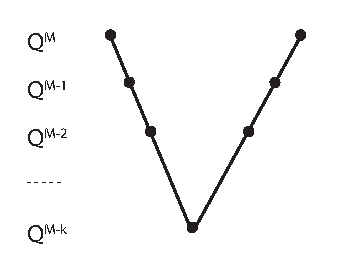
\includegraphics[height=41mm]{img/vcycle.pdf}
\caption{V cycle}
\end{subfigure}
\begin{subfigure}[]{0.3\textwidth}
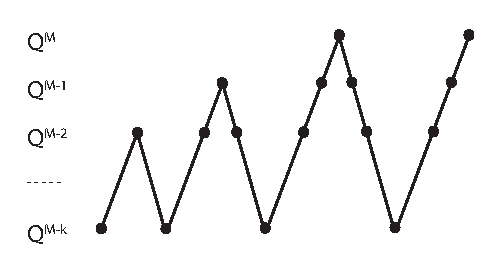
\includegraphics[height=41mm]{img/fullcycle.pdf}
\caption{Full cycle}
\end{subfigure}
\caption{The two different multigrid schemes presented in this report}
\label{multigrid}
\end{figure}
\noindent
Using restriction and prolongation operations on the pressure grid in the V-cycles act as a low pass filter and this an unwanted effect. Instead of moving the pressure solution from one resolution to another, we will use restriction on the residual $r^{M-n} = b^{M-n} - A^{M-n}p^{M-n}$ and prolongation on the pressure $p$. Instead of solving $Ap = b$ in each resolution, we solve $Ap = r$. To update the pressure of level $M-n$ we use the linear combination of $p^{M-n}$ and $prolong(p^{M-n-1})$.

\begin{equation}
p^{M-n}_{n+1} = p^{M-n}_n + prolong(p^{M-n-1})
\end{equation}

\begin{equation}
r^{M-n} = b^{M-n} - A^{M-n} p^{M-n}_n 
\end{equation}
\noindent
Equation \ref{multigridsplit} explains why using a linear combination of two different resolutions work in the V-cycle update.

\begin{equation}
\begin{split}
A^{M-n} p^{M-n}_{n+1} &= b^{M-n} \\
A^{M-n} (p^{M-n}_n + prolong(p^{M-n-1})) &= b^{M-n} \\
A^{M-n} prolong(p^{M-n-1}) +  \underbrace{ A^{M-n} p^{M-n}_n -  b^{M-n} }_\text{$-r^{M-n}$} &= 0 \\
A^{M-n} prolong(p^{M-n-1})  &= r^{M-n}
\end{split}
\label{multigridsplit}
\end{equation}
\noindent
If $M$ is the initial resolution number for the grid, we can specify a lower minimum resolution number $K$. For example, we do not want to solve the pressure equations for grids with dimension sizes small as $1$ and $2$.

\begin{algorithm}
\caption{Multigrid method}
\begin{algorithmic}[1]
\FOR{$m = M - 1$ down to $K$}
\STATE $\phi^m$ = restrict($\phi^{m+1}$)
\STATE $\phi^m_s$ = restrict($\phi^{m+1}_s$)
\ENDFOR

\FOR{$m = M$ down to $K$}
\STATE Build sparse matrix $A^m$
\ENDFOR

\STATE Build right hand side $b$
\STATE Initial guess $p^M = 0$

\FOR{i = 1 to $N_{\text{Full cycle}}$}
\STATE Full cycle
\ENDFOR

\FOR{i = 1 to $N_{\text{V cycle}}$}
\STATE V cycle(M)
\ENDFOR

\end{algorithmic}
\label{multigridalgorithm}
\end{algorithm}


\begin{algorithm}
\caption{V cycle(m)}
\begin{algorithmic}[1]

\FOR{i = 1 to $N_{\text{sweep}}$}
\STATE Gauss-Seidel to solve $A^mp^m = r^m$
\ENDFOR

\STATE $r^m = r^m - A^mp^m$
\STATE $r^{m-1} = restrict(r^m)$
\STATE $p^{m-1} = 0$
\STATE V cycle(m-1)
\STATE $p^m = p^m + prolong(p^{m-1})$

\FOR{i = 1 to $N_{\text{sweep}}$}
\STATE Gauss-Seidel to solve $A^mp^m = r^m$
\ENDFOR

\end{algorithmic}
\label{multigridalgorithm}
\end{algorithm}
\noindent
In Algorithms \ref{vcyclealgorithm}, \ref{vcyclealgorithm} and \ref{fullcyclealgorithm}, we only use the restriction operators on the surface tracking level set and the residuals. The prolongation operator is only used on the pressure grids. 

\begin{algorithm}
\caption{Full cycle()}
\begin{algorithmic}[1]

\STATE $p^{tmp} = p^M$
\FOR{m = K to M}
\IF{$m \neq K$}
\STATE $p^m = prolong(p^{m-1})$
\ENDIF
\STATE V cycle(m)

\ENDFOR

\STATE $p^M = p^{tmp} + p^M$

\end{algorithmic}
\label{fullcyclealgorithm}
\end{algorithm}
\noindent
We know have all the components we need to solve the pressure equations and make sure the velocity field is divergence free. There are three variables we can tweak in the multigrid method for performance and convergence rate. The first one, $N_{sweep}$, determines the number of Red Black Gauss-Seidel iterations in each resolution. The other two, $N_{\text{Full cycle}}$ and $N_\text{V cycle}$, decide how many times to run each cycle method. The \emph{Full cycle} converges faster in theory but in practice, all the restriction and prolongation operations can be expensive in an implementation. In general, the larger $N_{sweep}$ is, the smaller can $N_{\text{Full cycle}}$ and $N_\text{V cycle}$ be and vice versa. The most optimal choice of parameters is situational and how to automatically detect the different scenarios is beyond this thesis. 
